%-----------------------
% Title page
%-----------------------
\begin{titlepage}
  \centering

  \textsc{ELEC4630 Assignment 2}\\
  \vspace{9cm}

  \rule{\linewidth}{0.5pt}\\

  \vspace{1em}
  \LARGE\textsc{Question 2}\\
  \vspace{1em}

  \LARGE\uppercase{\textbf{{3D Reconstruction}}}\\

  \rule{\linewidth}{2pt}\\

  \vfill

  \normalsize{Deren Teo (4528554)}
  \vspace{1cm}

\end{titlepage}

%-----------------------
% Report body
%-----------------------
\section{Introduction}

Dense 3D reconstruction from multiple RGB images has long been a topic of interest in computer vision, and serves numerous practical purposes \cite{ulusoy_2016}. For example, 3D reconstruction applied to medical imaging can enable medical experts to better visualise areas of interest, for more accurate dianoses and better planning of medical procedures \cite{icoi_nd}. 3D reconstruction also has applications in a civil engineering context, to reconstruct models of buildings, roads, bridges, and other structures from 3D point clouds \cite{ma_2018}. One well-established technique for 3D reconstruction is shape-from-silhouette (SHS) \cite{cheung_2005}. SHS estimates a 3D reconstruction based on silhouettes of an object from multiple view points \cite{cheung_2005}. This report presents one attempt at using SHS to reconstruct the well-known Oxford Dinosaur using the standard data set of 36 images \cite{schoning_2015}.

\newpage
\section{Background Theory}

\subsection{Projective Geometry}

Projective geometry is a branch of mathematics concerned with the transforms associated with projecting geometric shapes onto a surface \cite{artmann_2018}. The concept is of foundational relevance to SHS because a silhouette is the projection of a shape in 3D space onto a 2D surface.

Consider the illustration of Figure \ref{fig:projective_geometry}, demonstrating the projection of a 3D object.

\begin{figure}[ht]
  \centering
  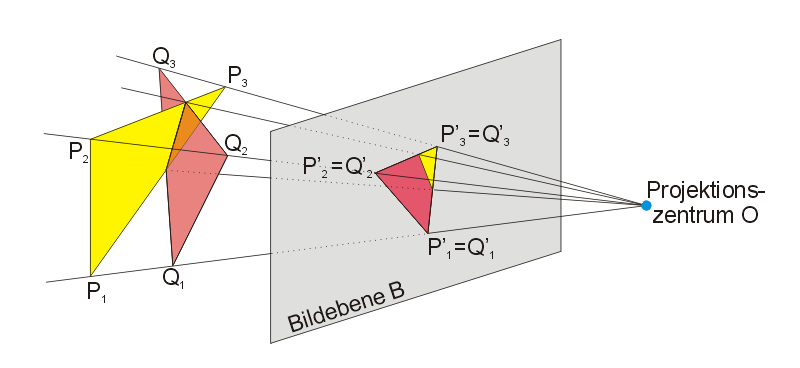
\includegraphics[width=0.6\textwidth]{images/q2_projective_geometry.jpg}
  \caption{Projection of a 3D object onto a 2D surface from a projection centre \cite{baecker_2005}.}
  \label{fig:projective_geometry}
\end{figure}

Intuitively, the projected image depends on the relative orientation of the surface and the object, and also on the distance between the projection centre and both the object and the surface. The orientation determines the projected image, and the distance defines the scale of the projection.

To capture the size of an object in a projection, since this varies with distance to the projection centre, projective geometry includes an additional coordinate, $w$, in addition to the standard Cartesian coordinates $x$ and $y$ (and $z$ in 3D space) \cite{lovell_2023b}. The additional coordinate specifies the distance between the projection and the projection centre \cite{lovell_2023b}.

Converting between projective and Cartesian coordinates in both 2D and 3D is simple \cite{lovell_2023b}:
\begin{align} \label{eqn:proj2cart}
  \text{In 2D: } (x, y, w) \longleftrightarrow \left( \frac{x}{w}, \frac{y}{w} \right) &&
  \text{In 3D: } (x, y, z, w) \longleftrightarrow \left( \frac{x}{w}, \frac{y}{w}, \frac{z}{w} \right)
\end{align}

Given the additional coordinate, $w$, if the pose of the projection centre is known, then it is possible to determine the size of the projected object.

Conversely, the projection of an object onto a surface can be calculated using a projective matrix, $P$. For the projection of a 3D object onto a 2D surface, the projective matrix has dimensions $3\times4$ \cite{lovell_2023b}, and internally captures all necessary information regarding the pose of the projection centre relative to the object.

Using projective coordinates, the projection of a point in 3D space relative to a surface and projection centre specified by some projection matrix is realised on the 2D surface as \cite{lovell_2023b}:
\begin{align} \label{eqn:projn}
  \begin{bmatrix}
    p_{11} & p_{12} & p_{13} & p_{14} \\
    p_{21} & p_{22} & p_{23} & p_{24} \\
    p_{31} & p_{32} & p_{33} & p_{34} \\
  \end{bmatrix}
  \begin{bmatrix}
    x \\
    y \\
    z \\
    w \\
  \end{bmatrix}
  =
  \begin{bmatrix}
    x_i \\
    y_i \\
    w_i \\
  \end{bmatrix}
\end{align}

In the inverse direction, however, given a projection centre pose, estimating the projection matrix is a non-trivial task \cite{lovell_2023b}. For the purposes of this investigation, projection matrices are known for all projections; therefore, no determination of projection matrices is necessary.

\newpage
\subsection{Shape-From-Silhouette}

Shape-from-silhouette (SHS) is a method of 3D reconstruction using silhouettes of an object as viewed from multiple known positions \cite{lovell_2023b}. In the nomenclature of projective geometry, a silhouette is a 2D projection of an object in 3D space, formed by the intersection of the visual cone of a ``camera'' at the projection centre \cite{cheung_2005}. Using a sufficient number of silhouettes from cameras with different relative poses, the 3D object can be approximately reconstructed as the intersection of the various visual cones \cite{lovell_2023b}. This is demonstrated by Figure \ref{fig:silhouettes}.

\begin{figure}[ht]
  \centering
  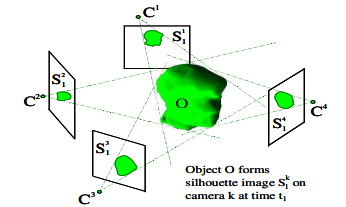
\includegraphics[width=0.5\textwidth]{images/q2_shape_from_silhouette.png}
  \caption{Silhouettes formed by the intersections of visual cones with a surface (from \cite{cheung_2005}).}
  \label{fig:silhouettes}
\end{figure}

The algorithm is programatically simple. The 3D reconstruction begins as a solid bounding box around the object of interest. Given a silhouette and an associated projection matrix, which defines the projective transformation between points in 3D space and points on the silhouette plane, each point in the reconstruction is projected onto the silhouette plane and compared with the silhouette. If the projected point lies outside the silhouette, then it is removed from the reconstruction. This is performed for all points in the reconstruction, and repeated for all available silhouettes. Once the algorithm concludes, the remaining shape is an approximate reconstruction of the original 3D object; the accuracy of the reconstruction depends on the number of silhouettes and the geometry of the object.

For example, Figure \ref{fig:shs_example} presents three SHS reconstructions of the same 3D model using an increasing number of silhouettes. The difference in reconstruction quality is evident.

\begin{figure}[ht]
  \centering
  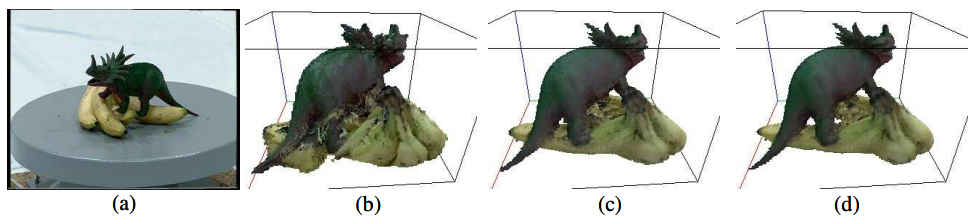
\includegraphics[width=0.8\textwidth]{images/q2_shape_from_silhouette_example.png}
  \caption{Coloured reconstructions of (a) using 6 (b), 36 (c), and 66 (d) silhouettes (from \cite{cheung_2005}).}
  \label{fig:shs_example}
\end{figure}

The advantages of SHS for 3D reconstruction include the easy availability of silhouettes, especially in an indoor environment with static cameras and controlled lighting \cite{cheung_2005}. For example, the Oxford Dinosaur dataset is derived from a single static camera capturing photographs at regular intervals of a dinosaur toy on a turntable. The colour of the photograph backgrounds makes it easy to segment a silhouette of the dinosaur.

However, SHS also has certain limitations. Foremost among these are that the quality of the reconstruction is highly dependent on the number of distinct silhouettes \cite{cheung_2005}. The method can also be sensitive to noise in segmented silhouettes \cite{lovell_2023b}. Finally, the method always produces a conservative reconstruction, and inherently cannot model convexities \cite{cheung_2005}.

\newpage
\section{Methodology}
\subsection{Silhouette Segmentation}

The SHS algorithm works on silhouettes, whereas the Oxford Dinosaur data set provides 36 colour images. Before applying SHS, the colour images must be converted into silhouettes. Fortunately, this is made intentionally easy by the data set designers; the images have sufficient and consistent lighting, and colour of the dinosaur contrasts strongly against the background.

Therefore, a silhouette can be extracted from each image by thresholding on hues:

\begin{enumerate}
  \item The image is converted into HSV and the hue channel is extracted.

  \item The hue image is first binarized using an experimentally-tuned lower threshold of 75.

  \item The hue image is again binarized using an experimentally-tuned upper threshold of 130.

  \item The binarized images are combined using a logical AND operation to preserve foreground.

  \item Border-connected white regions are cleared, removing the black strip on the right side.

\end{enumerate}

The procedure applies two thresholds to improve the segmentation accuracy of shadowed parts of the dinosaur, which take on a slightly blue hue due to reflection from the ground surface.

The lower threshold conservatively segments the background, losing detail of the shadowed parts of the dinosaur in the process. To restore the lost detail, the upper threshold segments only the shadowed parts of the dinosaur. Combining the two segmented results produces a complete segmentation of the dinosaur silhouette.

Figure \ref{fig:thresholds} presents an example of this procedure, as applied to the first image in the data set.

\begin{figure}[ht]
  \centering
  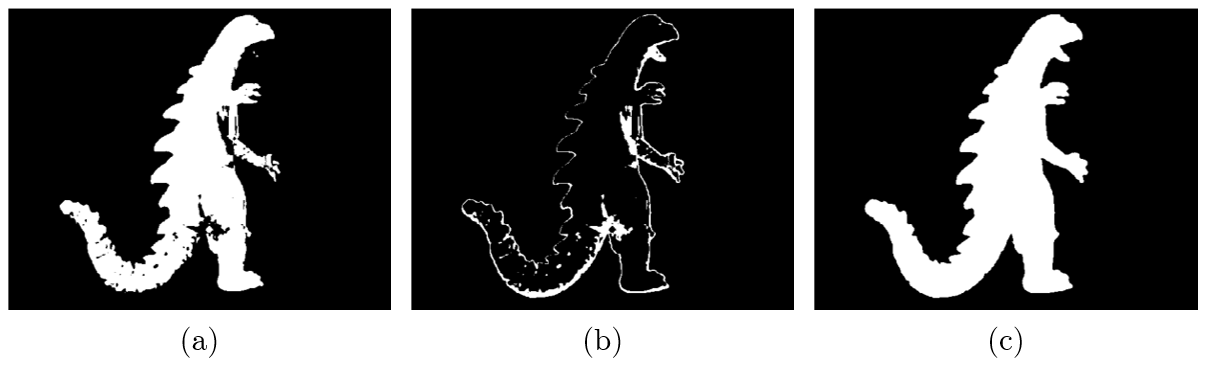
\includegraphics[width=0.7\textwidth]{images/q2_thresholds.png}
  \caption{Upper (a) and lower (b) thresholds of hue image produce a clean segmentation (c).}
  \label{fig:thresholds}
\end{figure}

It is likely that a similar result could be achieved by an adaptive threshold or morphology; however, this approach represents a sufficiently simple, fast and accurate solution.

\newpage
\subsection{Intuitive Shape-From-Silhouette}

Following silhouette segmentation, SHS can be applied to the data set. Two implementations are described: the first, an intuitive but inefficient approach, described in this section, and the second, a less intuitive but highly performant approach, described in the following section.

The intuitive approach implements SHS exactly as described in the presented theory. That is, for every silhouette, the algorithm iterates over every voxel in a pre-defined bounding volume and projects the voxels onto the silhouette. If the projection lies outside of the white silhouette region, then the voxel is marked as empty and not subsequently revisited. In this manner, voxels are ``carved away'' to iteratively refine the bounding volume into the dinosaur reconstruction.

To describe the process in more detail:

\begin{enumerate}
  \item A bounding volume is defined as a 3D array of size $270\times150\times440$. Each cell is a voxel; a value of 1 indicates a non-empty voxel, and 0 an empty voxel. All voxels begin non-empty.

  \item The first silhouette is processed by iterating over all non-empty voxels in the bounding volume. The voxels are first converted to projective coordinate form by appending a 1.

  \item This enables matrix multiplication of the voxel with the associated projection matrix, as per Equation \ref{eqn:projn}, yielding a 2D projective coordinate.

  \item The 2D projective coordinate represents a pixel on the silhouette plane. The coordinate is converted to Cartesian form by dividing the first two entries by the last.

  \item The coordinate is rounded down to the nearest integer, to enable comparison with pixels in the silhouette image.

  \item If the coordinate does not coincide with a white silhouette region, the projected voxel is marked as empty.

  \item Steps 3 to 6 are repeated for all non-empty voxels in the volume.

  \item Steps 2 to 7 are repeated for all remaining silhouettes.

\end{enumerate}

While this approach is intuitive, it is easy to see the inefficiency of the method. Consider the number of voxels in the initial bounding volume: $270\times150\times440=17,820,000$.

One at a time, each voxel is projected onto a silhouette. Given there are 36 silhouettes, the innermost loop (there are four in total) is entered: $18,046,141\times36=641,520,000$ times.

While the fact that empty voxels are not re-evaluated no doubt decreases the run time, a full execution still exceeds 30 minutes on a reasonably powerful desktop computer. This proves infeasible for tuning and debugging; hence, an alternative implementation is developed.

\newpage
\subsection{Optimised Shape-From-Silhouette}

To decrease the run time of the SHS algorithm, an optimised approach is implemented based on the SpaceCarving program by Zins \cite{zins_2019}. The approach makes extensive use of NumPy array operations, which are highly optimised. The resulting SHS implementation runs a full execution in approximately 50 seconds, representing an impressive speed improvement of over 97\%.

However, to use the matrix operations, the majority of data structures used for the intuitive implementation are entirely revised, obfuscating the intuition to a degree.

The optimised implementation follows the following procedure:

\begin{enumerate}
  \item A voxel array of 3D projective coordinates is constructed, representing the coordinates of each voxel in the initial bounding volume. That is, the array has dimensions $4\times N$, where $N$ is the number of voxels in the bounding volume (i.e. $17,820,000$).

  \item The first silhouette is processed by multiplying the associated projection matrix with the voxel array, yielding all 2D projective coordinates simultaneously.

  \item The new pixel array of 2D projective coordinates, representing pixels on the silhouette plane, is converted to Cartesian form by dividing the first two columns by the last.

  \item The 2D coordinates are rounded to the nearest integer, to enable comparison with pixels in the silhouette image.

  \item Each coordinate in the pixel array is checked against the bounds of the silhouette image. Coordinates not within the image dimensions are discarded before continuing.

  \item Each remaining projected pixel is compared with the silhouette image simultaneously, by using the pixel array to index into the image.

  \item The comparison results for each projected pixel are recorded in a 1D array as either empty or non-empty. The recorded array is bijectively associated with the initial voxel array.

  \item Steps 2 to 7 are repeated for the remaining silhouettes.

  \item After processing all silhouettes, the result is a number of 1D arrays containing voxel states from the perspective of each silhouette. The arrays are compressed into a single dimension such that any voxel which appears empty in any silhouette is decided as empty.

  \item By matching the voxel array to the voxel states array, a reconstruction is thus obtained.

\end{enumerate}

The speed improvement of this implementation is largely attributable to Step 2 above. Rather than iterating over all voxels sequentially, the construction of the voxel array enables all voxels to be projected simultaneously in one highly optimised matrix operation. Similar is true for Step 6, wherein the states of the projected voxels are determined in one indexing operation.

The result of this implementation is exactly the same as for the intuitive implementation, yet the use of optimised matrix operations enables a speed-up of, as mentioned, over 97\%. Perhaps the only disadvantage of this implementation is that it is is decidely less intuitive to program, and hence debug.

\newpage
\section{Results}

Figure \ref{fig:dino_views} presents four new views of the dinosaur as reconstructed using the SHS algorithm and viewed using the ParaView 5.11.1 software \cite{kitware_2023}.

\begin{figure}[ht]
  \centering
  \begin{subfigure}[b]{0.4\textwidth}
    \centering
    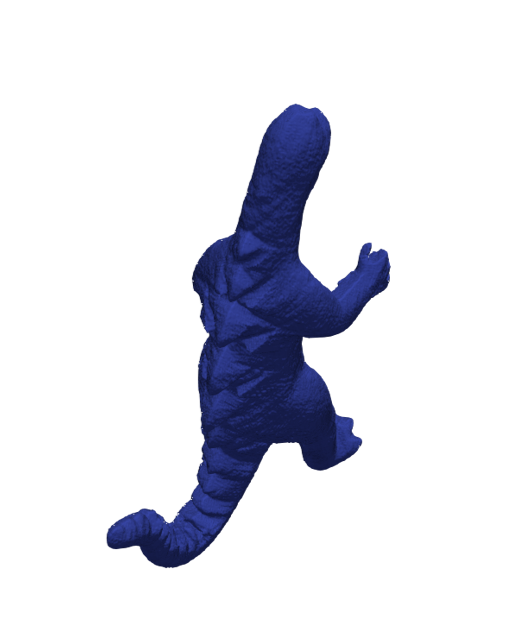
\includegraphics[width=\textwidth]{images/q2_dino_view_1.png}
    \caption{}
  \end{subfigure}
  \hspace{1em}
  \begin{subfigure}[b]{0.4\textwidth}
    \centering
    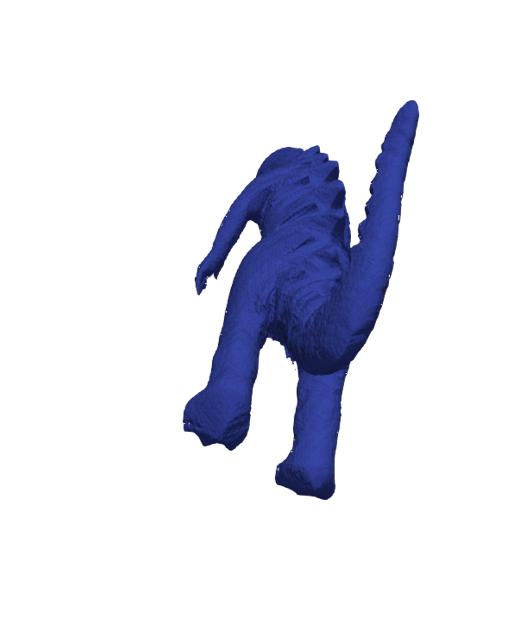
\includegraphics[width=\textwidth]{images/q2_dino_view_2.png}
    \caption{}
  \end{subfigure}
  \\
  \begin{subfigure}[b]{0.4\textwidth}
    \centering
    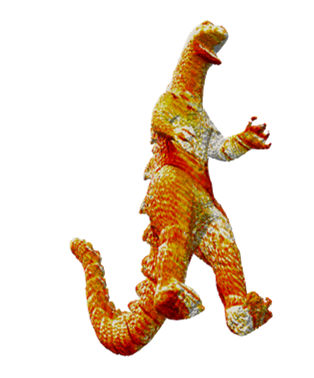
\includegraphics[width=\textwidth]{images/q2_dino_view_3.png}
    \caption{}
  \end{subfigure}
  \hspace{1em}
  \begin{subfigure}[b]{0.4\textwidth}
    \centering
    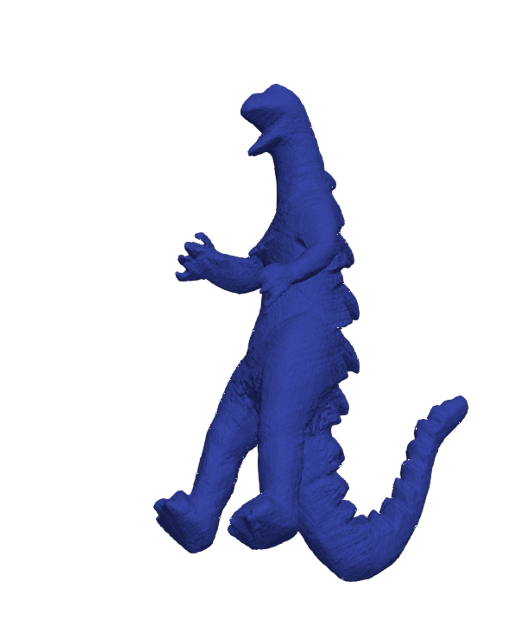
\includegraphics[width=\textwidth]{images/q2_dino_view_4.png}
    \caption{}
  \end{subfigure}
  \caption{Four views of the reconstructed dinosaur, not coinciding with data set views.}
  \label{fig:dino_views}
\end{figure}

\newpage
\section{Discussion}

This report has presented two implementations of the shape-frome-silhouette (SHS) algorithm: an intuitive but inefficient implementation, and a less intuitive but highly performant implementation. The latter is applied to reconstruct a model of the well-known Oxford Dinosaur, from the original data set of 36 images. The solution successfully reconstructs the dinosaur to an expected degree of accuracy, and demonstrates some advantages and disadvantages of the SHS algorithm.

Foremost among the advantages of the SHS algorithm is the easy availability of silhouettes, especially in a controlled environment \cite{cheung_2005}. This is demonstrated by the high segmentation accuracy achievable on the Oxford Dinosaur data set, enabled by consistent and high quality lighting and a background chosen to contrast strongly with the dinosaur foreground. The segmentated first image is provided as an example in the methodology.

On the other hand, this advantage arguably only compensates for the simultaneous sensitivity of the algorithm to segmentation accuracy \cite{lovell_2023b}. This sensitivity arises from the practice of clearing voxels which appear empty in any silhouette. As a result, if any silhouette is improperly segmented, parts of the model may erroneously appear empty and be cleared, which by design will not be rectified by any subsequent process.

A remedy to this, as implemented by the SpaceCarving implementation of Zins \cite{zins_2019}, is to instead capture a count of the number of viewpoints perceiving each voxel as non-empty. If this count exceeds some threshold, then the voxel is considered non-empty. This is a conservative approach to SHS, which affords some tolerance to segmentation errors. However, the accuracy of the reconstruction is notably inferior, resulting in erroneous protrusions when applied to the Oxford Dinosaur problem.

A further limitation, conceivably greater than just discussed, is that the quality of the reconstruction is highly dependent on the number of distinct silhouettes \cite{cheung_2005}. This is demontrated by Figure \ref{fig:shs_example} in the theory section, from Cheung et. al \cite{cheung_2005}, and a similar example is presented in Figure \ref{fig:bad_reconstruction} for the Oxford Dinosaur model.

\begin{figure}[ht]
  \centering
  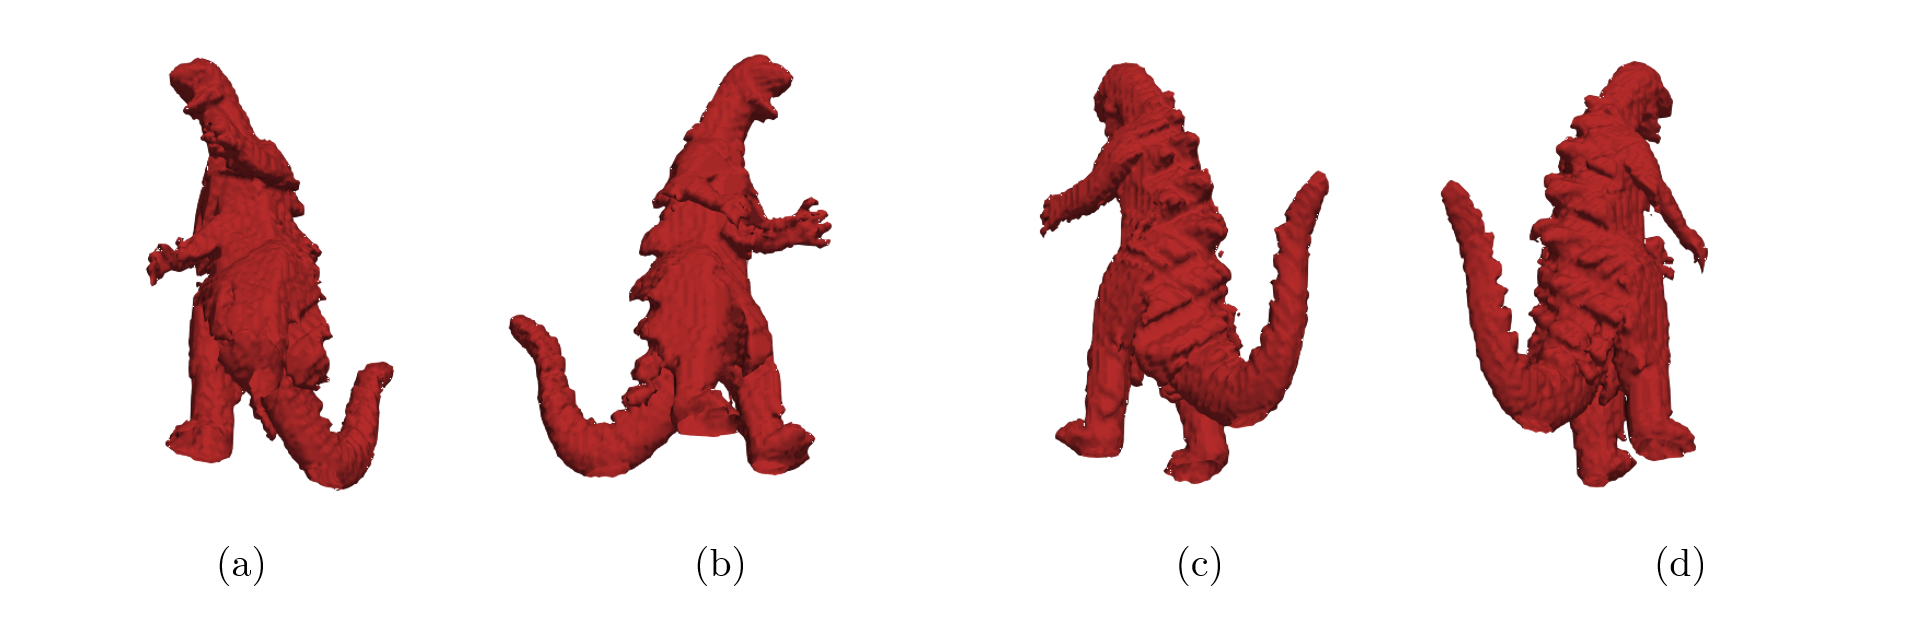
\includegraphics[width=0.9\textwidth]{images/q2_bad_reconstruction.png}
  \caption{Reconstruction of the Oxford Dinosaur using only six silhouettes.}
  \label{fig:bad_reconstruction}
\end{figure}

Figure \ref{fig:bad_reconstruction} presents the SHS reconstruction of the Oxford Dinosaur using only every sixth silhouette; the result may be compared to Figure \ref{fig:dino_views} and the significant difference observed. This limitation is inherent to the SHS method, and is particularly consequential for scenarios where a practitioner may have access only to a limited existing set of images or silhouettes. This may occur, for example, in medical imaging. If in addition to this, the silhouettes are not, or cannot be, accurately segmented, then the SHS reconstruction will have a very limited quality.

\section{Conclusion}

In summary, this report presents an implementation of the shape-from-silhouette algorithm, and the result it achieves in reconstructing the Oxford Dinosaur. The result demonstrates advantages and limitations of the shape-from-silhouette algorithm. Notably, a discussion is founded surrounding the sensitivity of the algorithm to segmentation accuracy, and the necessity of a sufficient number of distinct silhouettes.
